%===================================== CHAP 4 =================================

\chapter{Platform (?)}

In 2016, the long anticipated new hardware was finally installed and was ready
to be used for the CARP project. The new machine contains four Convey Wolverine
Application Accelerators, coprocessors aimed at accelerating key parts of
algorithms in high-performance computing through reconfigurable hardware. Each
accelerator is equipped with a state-of-the-art Xilinx FPGA and large,
high-bandwidth on-chip memory.

The following sections describe the Wolverine accelerator architecture, the
toolchain used to synthesize the hardware design and finally the toolchain used
for the software API.

\section{Convey Wolverine WX-2000 Application Accelerator}

The Convey Wolverine WX-2000 is a PCIe-mounted coprocessor equipped with a
Xilinx Virtex-7 XC7V2000T FPGA and four SO-DIMM slots allowing for up to 64 GB
of on-chip memory. \figurename~\ref{fig:convey-wx-card} shows how a Wolverine
coprocessor is organized at a high level. The host computer communicates with
the card over PCIe at a max bandwidth of 8 GB/s. On the coprocessor the Host
Interface controller (HIX) is responsible for decoding the data sent from the
host. Data can either be stored in the on-board memory, or passed directly to an
the FPGA.

With 2 million logic cells, 46 MB of BRAM and up to 2.8 Tb/s serial bandwidth,
the XC7V2000T is one of Xilinx' higher end FPGAs. Earlier, FPGAs have been
scaled monolithically following Moore's Law \todo{reference}, in the same way
conventional processors have been scaled. With the XC7V2000T however, Xilinx has
opted to combine 4 separate dies into one large virtual FPGA with their Stacked
Silicon Interconnect (SSI) technology \cite{Saban2011}. Each die, or Super Logic
Region (SLR), has its own clocking and configuration circuitry. For monolithic
designs, these signals would have to be routed throughout the entire die in
complex ways to avoid critical paths that are too long. With this circuitry
replicated in each SLR, the resources required for routing clocking and
configuration signals is significantly lower, opening up the possibility to use
these resources to interconnect the SLRs instead. This, along with advances in
manifacturing techniques has allowed Xilinx to scale their FPGAs in news and
opening up new use cases for them. Programming FPGAs using SSI is no different
from any other FPGA, the Xilinx design flow toolchain distributes designs across
multiple SLRs if needed.


\begin{figure}[ht]
  \centering
  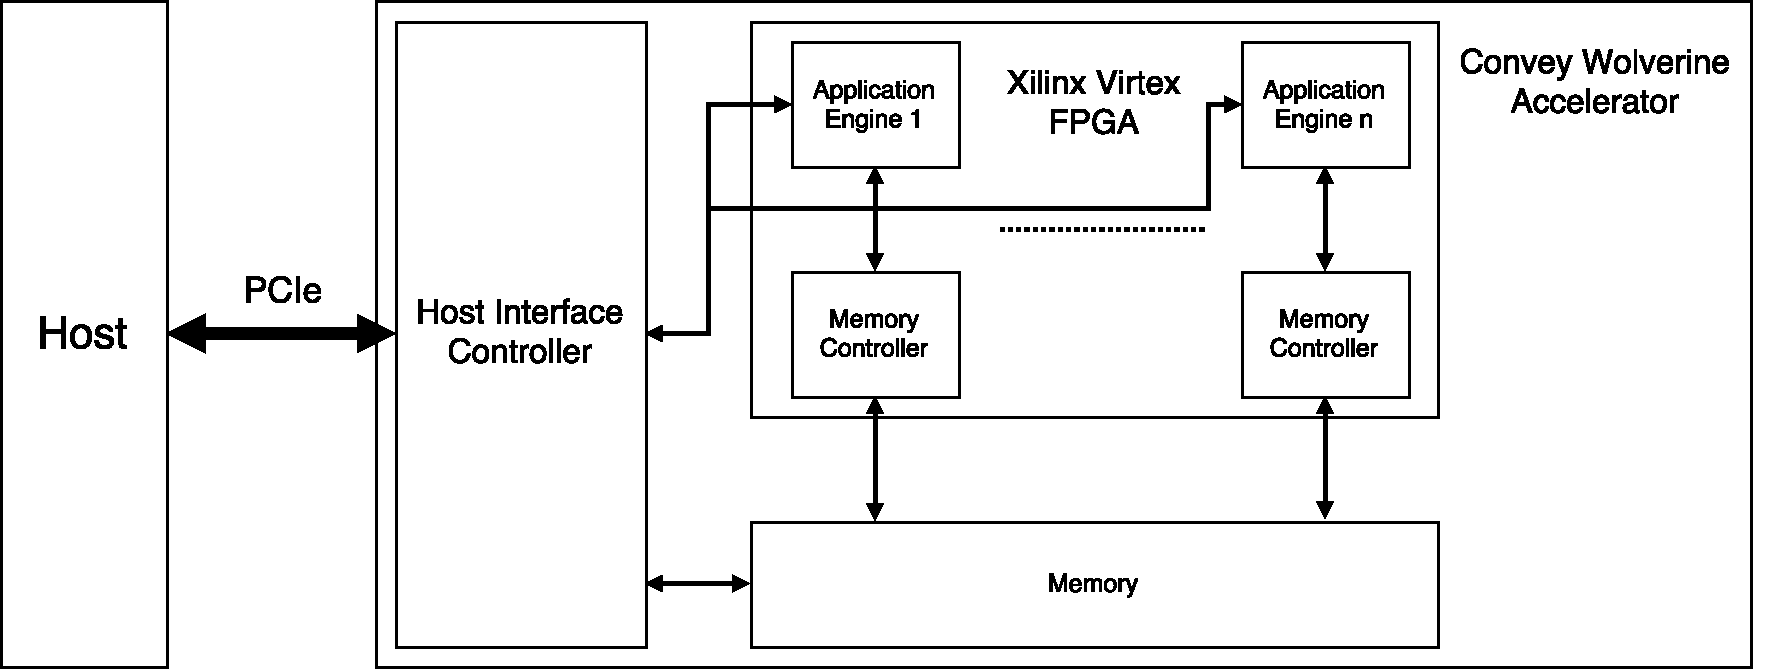
\includegraphics[width=\linewidth]{fig/convey-wx-card}
  \caption{
    High level overview of the Convey Wolverine Accelerator architecture.
    \label{fig:convey-wx-card}
  }
\end{figure}


\section{Hardware Toolchain}


\subsection{Scala/Chisel}

\section{Software Toolchain}


\cleardoublepage
%%% Local Variables:
%%% mode: latex
%%% TeX-master: "../thesis"
%%% End:
